
\section{Ugeopgave 1}
\label{sec:ugeopgave-1}

Form�let med denne opgave var at blive introduceret til at lave,
redigere, linke og k�re C- og C++-programmer, der er bruger OpenGL,
GLU og GLUT.

\subsection{Del 1}
\label{sec:del-1}

Programmet, n�r det k�res, viser vinduet i figur \ref{fig:1-1}.

\begin{figure}[hp]
\centering
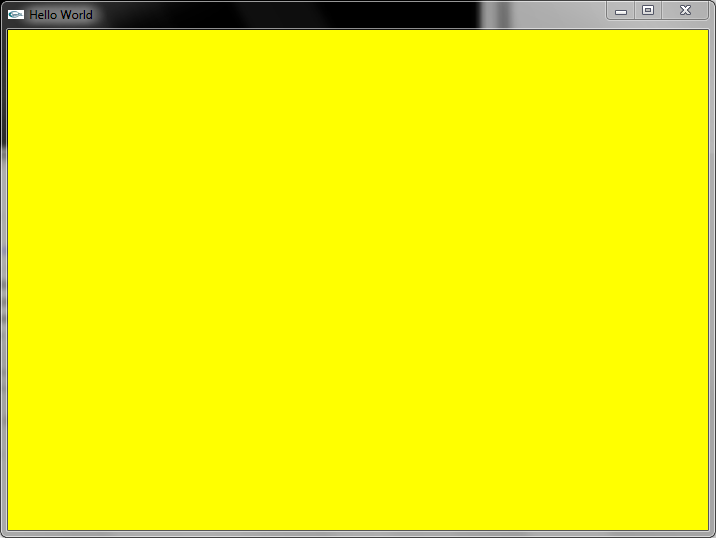
\includegraphics[width=8cm]{../exercise1/part1/screenshots/part1_1.png}
\caption{F�rste k�rsel}
\label{fig:1-1}
\end{figure}

N�r der tilf�jes de udkommenterede linjer, bliver koordinatsystemet
sat, s� man kan se den gule polygon i sin fulde udstr�kning p�
sk�rmen. Det kan ses p� figur \ref{fig:1-2}.

\begin{figure}[hp]
\centering
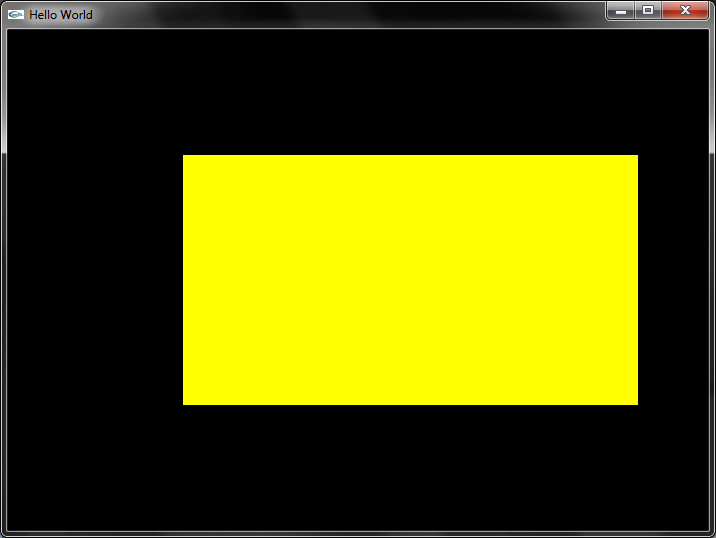
\includegraphics[width=8cm]{../exercise1/part1/screenshots/part1_2.png}
\caption{Tilf�jelse af udkommenterede linjer}
\label{fig:1-2}
\end{figure}

\subsection{Del 2}
\label{sec:del-2}

Programmet, n�r det k�res, viser vinduet i figur \ref{fig:2-1}.
%
Dern�st blev der tilf�jet en r�d trekant, med knuderne $(2,2)$,
$(5,2)$ og $3.5,5)$. Dette kan ses p� figur \ref{fig:2-2}.
%
Trekanten er herefter translateret med vektoren $(6,7)$. Det ses p�
figur \ref{fig:2-3}.
%
Efterf�lgende er de enkelte hj�rner i trekanten blevet farve
henholdsvis r�d, gr�n og bl�. Det ses p� figur \ref{fig:2-4}.
%
Rektanglet er herefter blevet roteret 45 grader mod uret om sin egen
midte. Dette er gjort ved at translatere rektanglet, s� dets midte var
i $(0,0)$ og derefter rotere om en akse. Resultatet ses p� figur \ref{fig:2-5}.

\begin{figure}[hp]
\centering
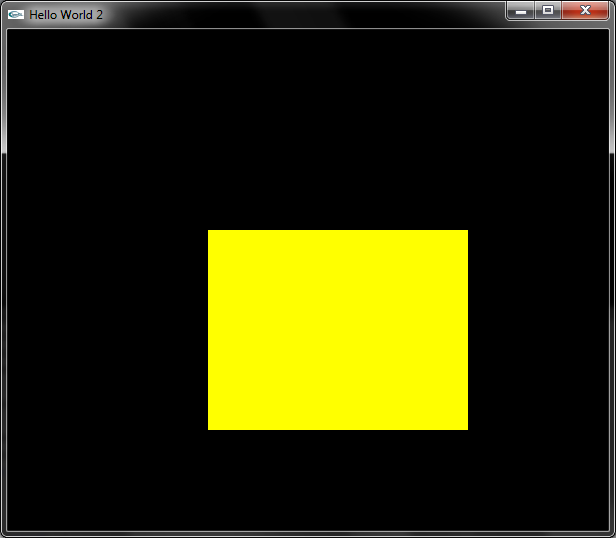
\includegraphics[width=8cm]{../exercise1/part2/screenshots/part2_1.png}
\caption{F�rste k�rsel}
\label{fig:2-1}
\end{figure}

\begin{figure}[hp]
\centering
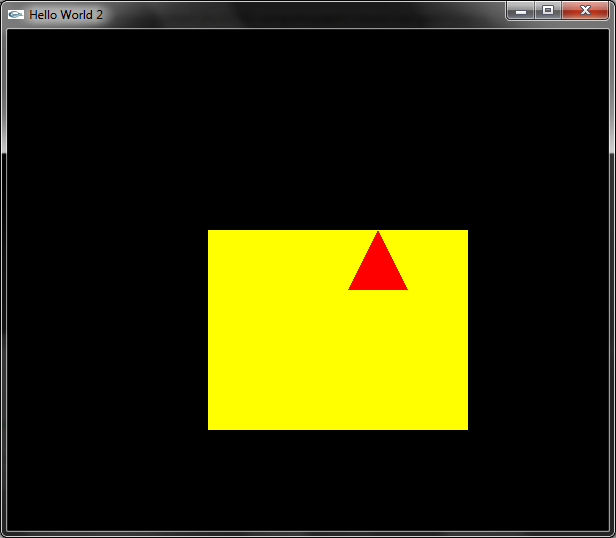
\includegraphics[width=8cm]{../exercise1/part2/screenshots/part2_2.png}
\caption{Tilf�jelse af en trekant}
\label{fig:2-2}
\end{figure}

\begin{figure}[hp]
\centering
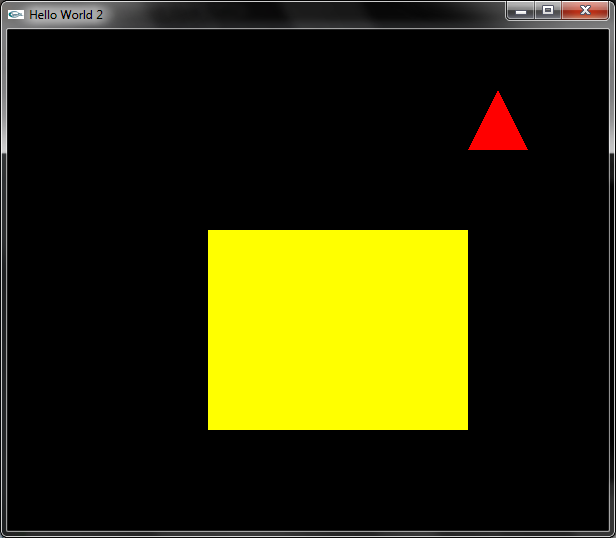
\includegraphics[width=8cm]{../exercise1/part2/screenshots/part2_3.png}
\caption{Translatering af trekant}
\label{fig:2-3}
\end{figure}

\begin{figure}[hp]
\centering
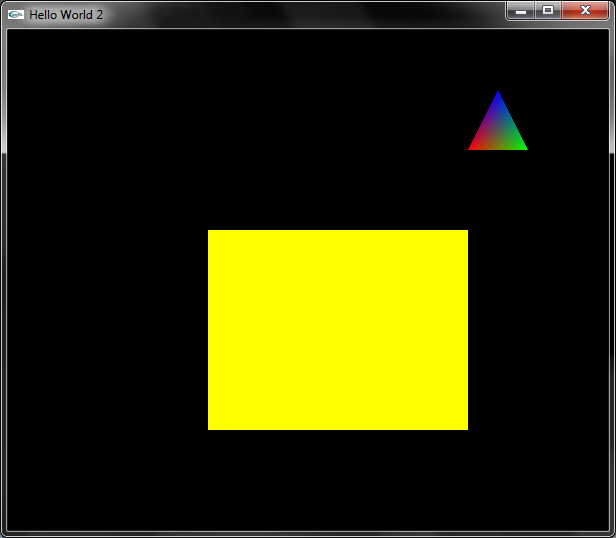
\includegraphics[width=8cm]{../exercise1/part2/screenshots/part2_4.png}
\caption{Omfarvning af trekant}
\label{fig:2-4}
\end{figure}

\begin{figure}[hp]
\centering
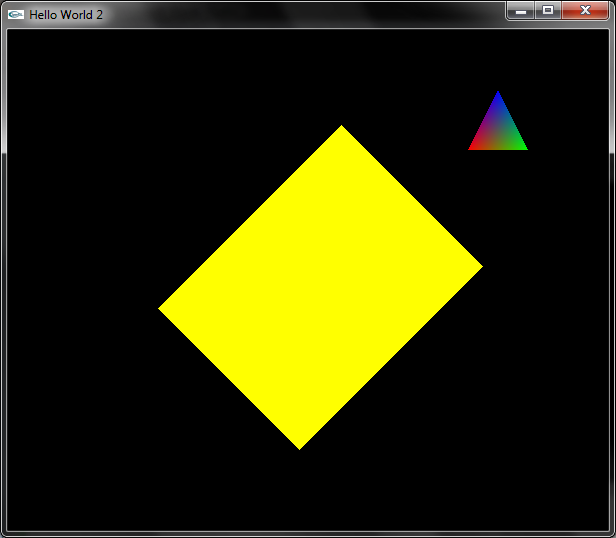
\includegraphics[width=8cm]{../exercise1/part2/screenshots/part2_5.png}
\caption{Rotering af rektangel}
\label{fig:2-5}
\end{figure}

%%% Local Variables: 
%%% mode: latex
%%% TeX-master: "report_main"
%%% End: 